\section{kubernetes基本组成}
kubernetes主要分为2种角色:master和node。其中,master包含了kube-apiserver,kube-scheduler和
kube-controller-manager;而node则包含了kubelet和kube-proxy。当然,可以把master和node节点混合
在一起。每个服务的角色和用途不一样。
\begin{itemize}
    \item kube-apiserver:提供api访问请求控制,访问etcd和转发etcd的访问控制请求。用户自己做Active-Active模式。
    \item kube-scheduler:负责pod的调度。默认Active-Backend模式
    \item kube-controller-manager:包含Node,route,service和volume等控制器。默认Active-Backend模式
    \item kubelet:控制pod(容器)。只负责当前节点,单点。
    \item kube-proxy:负责为Service提供cluster内部的服务发现和负载均衡。只负责当前节点,单点。
\end{itemize}

创建一组pod时,其内部大致流程如图 \nameref{fig:create_pod}所示
\begin{figure}[H]
  \centering
  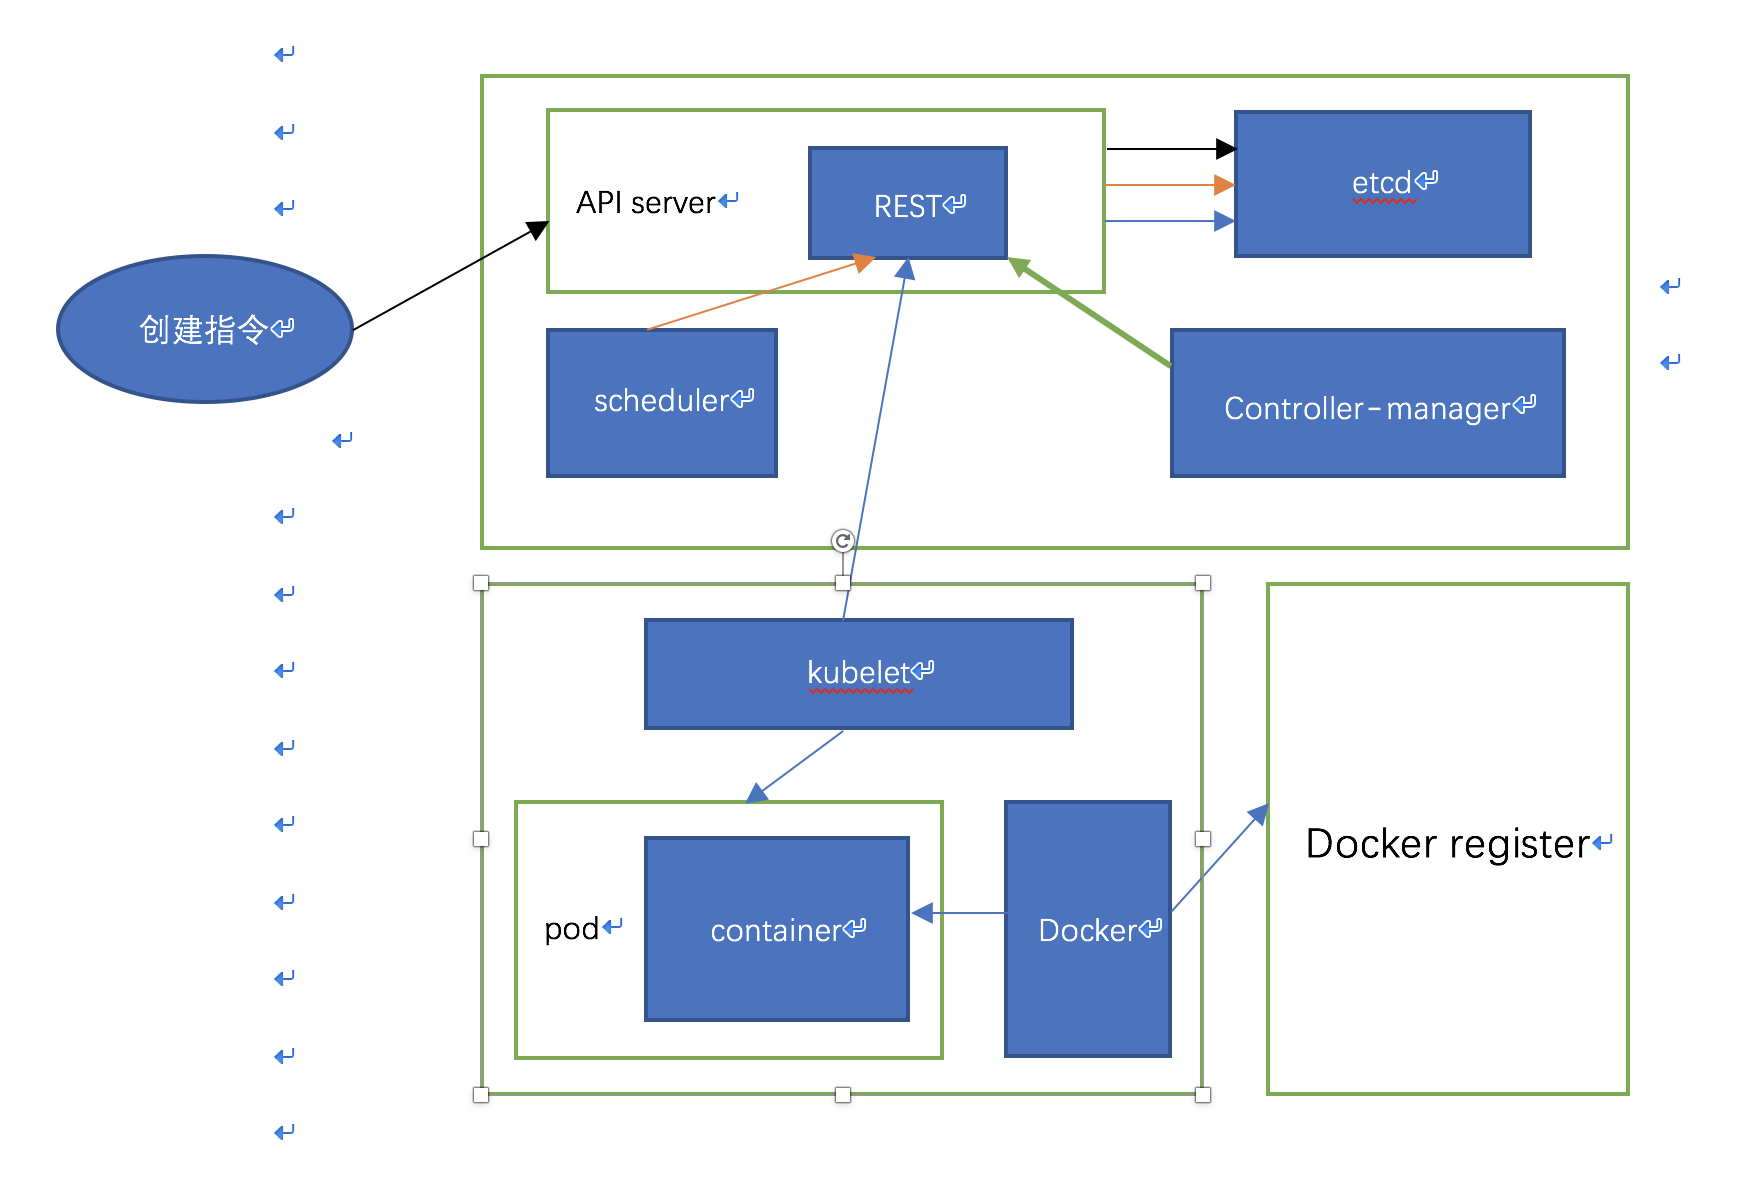
\includegraphics[scale=0.5]{create_pod.png}
  \caption{新建pod}
  \label{fig:create_pod}
\end{figure}

\begin{enumerate}
    \item 指令传到APIserver,API server将pod的创建信息固化到etcd上
    \item scheduler监控APIserver的watch端口,查看到etcd中有创建pod的消息,下面就为pod选择合适的node节点,并进行绑定,绑定成功后,scheduler会调用APIServer的API的增加接口在etcd中创建一个boundpod对象,描述在一个工作节点上绑定运行的所有pod信息
    \item kubelet监控APIserver的watch端口监听pod信息,发现有新的pod绑定在该节点上的时候,则根据etcd中的boundpod信息进行pod创建
    \item docker会从image仓库中查看docker的信息,并下载docker image最终进行container的创建
    \item controller-manager会监听API server的端口,对node、pod副本、资源等进行管理
\end{enumerate}

而通过外部访问pod时,其内部流程又存在一些区别,其大致如图\nameref{fig:visit_pod}所示
\begin{figure}[H]
    \centering
    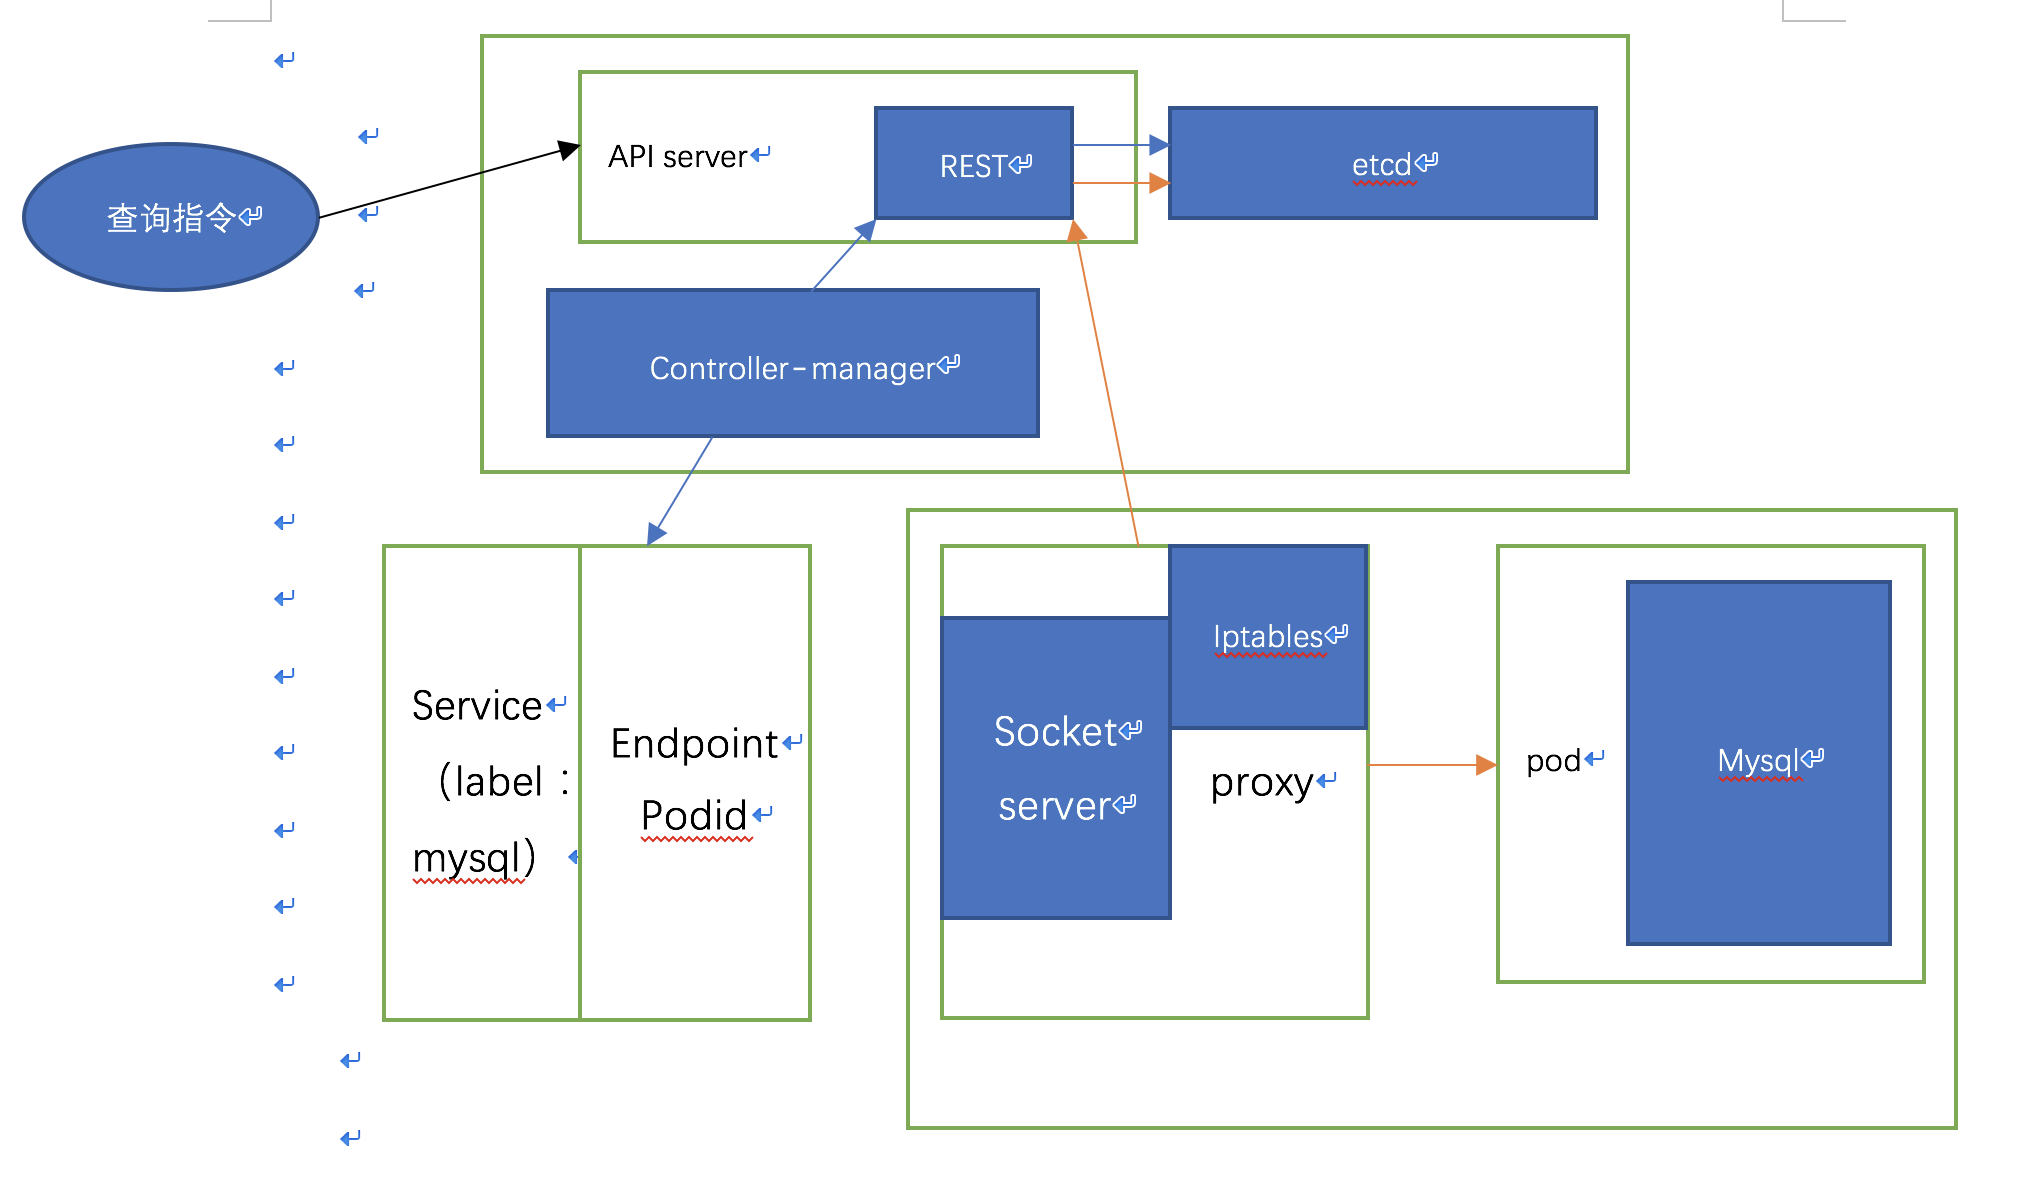
\includegraphics[scale=0.4]{visit_pod.png}
    \caption{访问pod}
    \label{fig:visit_pod}
\end{figure}
\begin{enumerate}
    \item controller-manager会监控API server的端口,然后管理service和endpoint的创建,其中endpoint主要是提供了server对应pod 的副本的访问地址
    \item proxy是service的主要实现者,他通过监听API server的端口,发现service,为service创建一个代理接口socket server用来接收来自server的访问请求,并创建Iptables,利用其规则使service的请求重定向到socket server。
    \item 在收到service请求之后,proxy将请求转发到后端的pod上,实现请求并实现负载均衡
\end{enumerate}

\section{kubernetes基本操作}

\subsection{NameSpace}
\begin{code-block}{bash}
# 查看所有namespace
kubectl get namespace
# 查看所有namespace,并包含lable信息
kubectl get namespace --show-labels
# 查看namespace的详细信息
kubectl describe namespace kube-system
# 从命令行新建namespace
kubectl create namespace zhangjl

# 从文件创建namespace
cat >zhangjl.yml<<EOF
apiVersion: v1
kind: Namespace
metadata:
  name: zhangjl
EOF
kubectl create -f zhangjl.yml

# 新建带有lable的namespace
cat >zhangjl.yml<<EOF
apiVersion: v1
kind: Namespace
metadata:
  name: zhangjl
  labels:
    namespace-name: zhangjl
    owner: zhangjl
EOF
kubectl create -f zhangjl.yml
\end{code-block}

\subsection{Context}
\begin{code-block}{bash}
# 获取所有上下文环境
kubectl config get-contexts

# 查看context的具体信息
kubectl config view

# 查看当前使用的context
kubectl config current-context

# 新增context
kubectl config set-context zhangjl --namespace=zhangjl --cluster=kubernetes --user=admin

# 切换至新的context
kubectl config use-context zhangjl

\end{code-block}

\subsection{Label}
\begin{code-block}{bash}
# 查看对象的label
kubectl get namespace --show-labels
kubectl get pod -o wide --show-labels

# 为对象添加label.label的添加可以多次进行。overwrite表示,如果对应的key存在,就进行更新,
# 否则进行创建
kubectl label namespace zhangjl ns-name=zhangjl name=zhangjl --overwrite
kubectl label pod zhangjl ns-name=zhangjl user=zhangjl --overwrite

# 删除label
kubectl label namespace zhangjl ns-name- name-
kubectl label pod zhangjl ns-name- name-

# 根据label进行搜索
kubectl get pod --all-namespaces  -l k8s-app==dashboard
kubectl get pod --all-namespaces  -l k8s-app!=dashboard

# selector 搜索
kubectl get pod --all-namespaces  -l 'k8s-app in (dashboard,default-http-backend)'
kubectl get pod --all-namespaces --selector='k8s-app==calico-kube-controllers'

# 多label搜索
kubectl get pod --all-namespaces  -l k8s-app!=dashboard,k8s-app==default-http-backend

# 混用selector和等式搜索
kubectl get pod --all-namespaces  -l 'k8s-app notin (dashboard,kube-dns), k8s-app==default-http-backend'
kubectl get pod --all-namespaces  --selector='k8s-app notin (dashboard,kube-dns), k8s-app==default-http-backend'
\end{code-block}
特别需要注意的是,node的label会影响pod的调度,pod的label会影响service和deployment等资源的选择。
另外,kubernetes当中,内置了很多label,具体的如下:
\begin{itemize}
    \item kubernetes.io/hostname
    \item failure-domain.beta.kubernetes.io/zone
    \item failure-domain.beta.kubernetes.io/region
    \item beta.kubernetes.io/instance-type
    \item beta.kubernetes.io/os
    \item beta.kubernetes.io/arch
\end{itemize}

\subsection{Pod}
\begin{code-block}{bash}
# 获取所有pod
kubectl get --all-namespace pod

# 展示pod的详情
kubectl describe --namespace=kube-system pod zhangjl

# 显示pod的日志
kubectl logs --namespace=kube-system zhangjl

# 指定namespace,并且指定node的label进行pod创建
cat >pod.yml<<EOF
apiVersion: v1
kind: Pod
metadata:
  name: nginx
  labels:
    env: test
    k8sapp: nginx
  namespace: zhangjl # 限定pod所在的namespace
spec:
  containers:
  - name: nginx
    image: nginx
    imagePullPolicy: IfNotPresent
  nodeSelector: # nodeSelector调度指令将在之后的版本进行废弃,使用affinity/anti-affinity代替
    disk_type: ssd # 指定pod所使用的磁盘类型
EOF
kubectl create -f pod.yml

# 使用anti-affinity/affinity进行pod的节点指定
# 根据node的亲和性与反亲和性进行调度
cat>pod.yml<<EOF
apiVersion: v1
kind: Pod
metadata:
  name: nginx
  labels:
    env: test
    k8sapp: nginx
    rules: node-affinity
  namespace: zhangjl
spec:
  containers:
  - name: nginx
    image: nginx
    imagePullPolicy: IfNotPresent
  affinity:
    nodeAffinity:
      requiredDuringSchedulingIgnoredDuringExecution:
        nodeSelectorTerms:
        - matchExpressions:
          - key: kubernetes.io/hostname
            operator: In
            values:
            - k8s1
            - k8s3
      preferredDuringSchedulingIgnoredDuringExecution:
      - weight: 1
        preference:
          matchExpressions:
          - key: disk_type
            operator: In
            values:
            - nvme
EOF

kubectl create -f pod.yml

# 根据pod的亲和性与反亲和性进行调度
# 在pod层面进行调度,比较的对象是节点上已经存在的
# pod。如果节点上没有pod,则该节点不在调度的考虑范围内。
cat>pod-affinity-pod.yml<<EOF
apiVersion: v1
kind: Pod
metadata:
  name: with-pod-affinity
  labels:
    affinity-rule: on_pod_level
  namespace: zhangjl
spec:
  affinity:
    podAffinity:
      # 要求调度之后的节点上,已经运行的pod当中,所有pod
      # 的label的k8sapp的值需要在nginx当中。强制性规则
      requiredDuringSchedulingIgnoredDuringExecution:
      - labelSelector:
          matchExpressions:
          - key: k8sapp
            operator: In
            values:
            - nginx
        topologyKey: kubernetes.io/hostname
    podAntiAffinity:
      # 希望调度之后的节点上,已经运行的pod当中,其label的env
      # 不在test当中。倾向性规则。
      preferredDuringSchedulingIgnoredDuringExecution:
      - weight: 100
        podAffinityTerm:
          labelSelector:
            matchExpressions:
            - key: env
              operator: NotIn
              values:
              - test
          topologyKey: kubernetes.io/hostname
  containers:
  - name: with-pod-affinity
    image: nginx
EOF

kubectl create -f pod-affinity-pod.yml
\end{code-block}
亲和性规则只针对pod和node。但是两者的规则是一致的。同样的,这些调度规则可以用于pod,replicate和deployment当中。
\begin{itemize}
    \item requiredDuringSchedulingIgnoredDuringExecution   必须满足,没有满足条件的node,pod会创建失败
    \item preferredDuringSchedulingIgnoredDuringExecution  尽力满足,没有满足条件的node,pod也会创建成功
    \item IgnoredDuringExecution的意思是,上面两条规则只在pod创建时起作用,如果pod已经运行,后来又改了node的lable,node不满足pod运行条件,但已经运行的pod不受影响
    \item requiredDuringSchedulingRequiredDuringExecution  现在不支持,后面版本会支持,作用基本等同requiredDuringSchedulingIgnoredDuringExecution,不同之处是pod改变label,对已经运行在其上的pod也会有影响。
\end{itemize}

\subsection{Secret}
Secret和认证相关,为用户的secret key。
\begin{code-block}{bash}
# 通过命令行创建secret key
echo -n 'admin' > ./username.txt
echo -n '1f2d1e2e67df' > ./password.txt
kubectl create secret generic db-user-pass --from-file=./username.txt --from-file=./password.txt

# 通过文件创建secret key
export user_name=`echo -n 'admin' | base64`
export pass_word=`echo -n '1f2d1e2e67df' | base64`
cat >secret.yml<<EOF
apiVersion: v1
kind: Secret
metadata:
  name: mysecret
type: Opaque
data:
  username: $user_name
  password: $pass_word
EOF

kubectl create -f secret.yml

# 查看secret详情
kubectl describe secret db-user-pass

# 透传secret key到pod当中
cat >secret-pod.yml<<EOF
apiVersion: v1
kind: Pod
metadata:
  name: secret-pod
  namespace: zhangjl
spec:
  containers:
  - name: secret-pod
    image: nginx
    volumeMounts:
    - name: secret-key
      mountPath: "/opt/secret-key"
      readOnly: true
  volumes:
  - name: secret-key
    secret:
      secretName: zhangjl
EOF
kubectl apply -f secret-pod.yml

# pod创建完毕之后,其内部的会在/opt/secret-key路径下
# 生成username和password文件,并且内容为解码之后的信息。

# 透传secret key的部分信息到pod当中
cat >secret-pod.yml<<EOF
apiVersion: v1
kind: Pod
metadata:
  name: secret-pod
  namespace: zhangjl
spec:
  containers:
  - name: secret-pod
    image: nginx
    volumeMounts:
    - name: secret-key
      mountPath: "/opt/secret-key"
      readOnly: true
  volumes:
  - name: secret-key
    secret:
      secretName: zhangjl
      items:             # 该标签标明只透传items下的内容,其他的信息不会进行透传
      - key: username
        path: user       # 将secret key当中的username透传到/opt/secret-key/user
                         # 而不是/opt/secret-key/username
EOF

# 以环境变量的方式使用secret key
cat >secret-env.yml<<EOF
apiVersion: v1
kind: Pod
metadata:
  name: secret-pod
  namespace: zhangjl
spec:
  containers:
  - name: secret-pod
    image: nginx
    env:
      - name: SECRET_USERNAME
        valueFrom:
          secretKeyRef:      # 表示secret key的引用
            name: zhangjl    # 引用的secret key的名称
            key: username
      - name: SECRET_PASSWORD
        valueFrom:
          secretKeyRef:
            name: zhangjl
            key: password
EOF
# 该文件apply之后,在容器内部进行env命令,即可搜索到对应的环境变量

# 修改host映射。该文件apply之后,在pod当中,hosts文件会有变化
# secret-pod指向了16.16.109.101
# kubectl exec hostaliases-pod -- cat /etc/hosts
cat >host-map.yml<<EOF
apiVersion: v1
kind: Pod
metadata:
  name: hostaliases-pod
  namespace: zhangjl
spec:
  hostAliases:
  - ip: "16.16.109.101"
    hostnames:
    - "secret-pod"
    - "secrete.remote"
  containers:
  - name: cat-hosts
    image: nginx
EOF

\end{code-block}

\subsection{Deployment}
1.7版本之前有replication的概念。目前,replication已经基本为deployment所取代,不复使用。
\begin{code-block}{bash}
# 创建简单的deployment
cat >deployment.yml<<EOF
# kubernetes 1.8
apiVersion: extensions/v1beta1
# kubernetes 1.10
#apiVersion: apps/v1
kind: Deployment
metadata:
  name: nginx-cluster
  namespace: zhangjl
spec:
  selector:
    matchLabels:
      run: nginx-cluster
  replicas: 2
  template:
    metadata:
      labels:
        run: nginx-cluster
    spec:
      containers:
      - name: nginx-cluster
        image: nginx
        ports:
        - containerPort: 80
EOF

# 利用node的affinity/anti-affinity进行调度
cat >node-affinity-deployment<<EOF
# kubernetes 1.8
apiVersion: extensions/v1beta1
# kubernetes 1.10
#apiVersion: apps/v1
kind: Deployment
metadata:
  name: nginx-cluster
  namespace: zhangjl
spec:
  selector:
    matchLabels:
      run: nginx-cluster
  replicas: 4
  template:
    metadata:
      labels:
        run: nginx-cluster
    spec:
      containers:
      - name: nginx-cluster
        image: nginx
        ports:
        - containerPort: 80
      affinity:
        nodeAffinity:
          requiredDuringSchedulingIgnoredDuringExecution:
            nodeSelectorTerms:
            - matchExpressions:
              - key: kubernetes.io/hostname
                operator: In
                values:
                - k8s1
                - k8s3
          preferredDuringSchedulingIgnoredDuringExecution:
          - weight: 100
            preference:
              matchExpressions:
              - key: disk_type
                operator: In
                values:
                - ssd
EOF

# 利用pod的affinity进行调度,将deployment的所有pod强制调度到
# 同一台node
cat >pod-affinity-deployment.yml<<EOF
# kubernetes 1.8
apiVersion: extensions/v1beta1
# kubernetes 1.10
#apiVersion: apps/v1
kind: Deployment
metadata:
  name: nginx-cluster
  namespace: zhangjl
spec:
  selector:
    matchLabels:
      run: nginx-cluster
      schedule: pod-affinity
  replicas: 3
  template:
    metadata:
      labels:
        run: nginx-cluster
        schedule: pod-affinity
        app: nginx-web-server
    spec:
      containers:
      - name: nginx-cluster
        image: nginx
        ports:
        - containerPort: 80
      affinity:
        podAffinity:
          requiredDuringSchedulingIgnoredDuringExecution:
          - labelSelector:
              matchExpressions:
              - key: app
                operator: In
                values:
                - nginx-web-server
            topologyKey: kubernetes.io/hostname
EOF

# 利用node-affinity和pod-affinity,将deployment的
# pod强制调度到k8s3
cat >pod-and-node-affinity-deployment.yml<<EOF
# kubernetes 1.8
apiVersion: extensions/v1beta1
# kubernetes 1.10
#apiVersion: apps/v1
kind: Deployment
metadata:
  name: nginx-cluster
  namespace: zhangjl
spec:
  selector:
    matchLabels:
      run: nginx-cluster
      schedule: pod-affinity
  replicas: 3
  template:
    metadata:
      labels:
        run: nginx-cluster
        schedule: pod-affinity
        app: nginx-web-server
    spec:
      containers:
      - name: nginx-cluster
        image: nginx
        ports:
        - containerPort: 80
      affinity:
        podAffinity:
          requiredDuringSchedulingIgnoredDuringExecution:
          - labelSelector:
              matchExpressions:
              - key: app
                operator: In
                values:
                - nginx-web-server
            topologyKey: kubernetes.io/hostname
        nodeAffinity:
          requiredDuringSchedulingIgnoredDuringExecution:
            nodeSelectorTerms:
            - matchExpressions:
              - key: kubernetes.io/hostname
                operator: In
                values:
                - k8s3
EOF

# 利用pod-anti-affinity,将deployment的pod调度到不同的节点上
cat >pod-anti-affinity-deployment.yml<<EOF
# kubernetes 1.8
apiVersion: extensions/v1beta1
# kubernetes 1.10
#apiVersion: apps/v1
kind: Deployment
metadata:
  name: nginx-cluster
  namespace: zhangjl
spec:
  selector:
    matchLabels:
      run: nginx-cluster
      schedule: pod-affinity
  replicas: 3
  template:
    metadata:
      labels:
        run: nginx-cluster
        schedule: pod-affinity
        app: nginx-web-server
    spec:
      containers:
      - name: nginx-cluster
        image: nginx
        ports:
        - containerPort: 80
      affinity:
        podAntiAffinity:
          requiredDuringSchedulingIgnoredDuringExecution:
          - labelSelector:
              matchExpressions:
              - key: app
                operator: In
                values:
                - nginx-web-server
            topologyKey: kubernetes.io/hostname
EOF
\end{code-block}

\subsection{Service}
Deployment只是指定了pod的副本数,调度规则,以及资源使用,但是并没有暴露对应的服务。如果是对外提供相关的服务,则
还需要创建service。需要注意的是,service可以独立存在,不依赖于pod。如果service需要的deployment和pod不存在,
service依然可以创建,只是service不可用而已。

另外需要注意的是,service和deployment创建的先后顺序会影响pod的env属性。
如果service先于deployment创建,则pod的env属性当中,会存在service的env,如图\nameref{fig:k8s_service}所示,
反之,则不存在。因此,操作顺序上一般是先创建service,再创建deployment。
\begin{figure}[H]
  \centering
  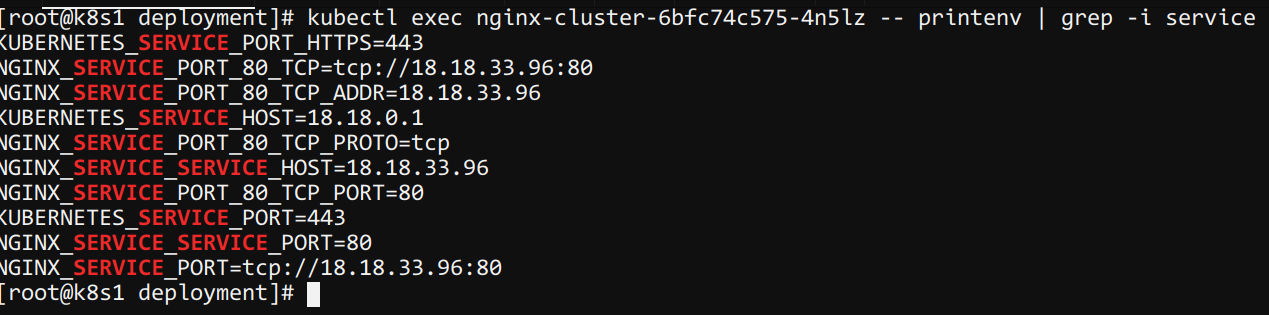
\includegraphics[scale=0.3]{k8s_service.png}
  \caption{新建service}
  \label{fig:k8s_service}
\end{figure}

\begin{code-block}{bash}
cat >service.yml<<EOF
apiVersion: v1
kind: Service
metadata:
  name: nginx-service
  labels:
    run: nginx-cluster
    schedule: pod-affinity
    service: nginx
spec:
  type: NodePort # 指定服务的暴露方式,采用NodePort方式
  ports:
  - port: 80        # 暴露的集群端口,供kubernetes集群内部访问
    targetPort: 80  # 容器内部暴露的端口
    nodePort: 31000 # 在node上暴露的端口,提供给外部访问
  selector: # 从deployment当中选择合适的deployment,deployment的metadata
            # 当中包含的一下的键值对
    run: nginx-cluster
    schedule: pod-affinity
EOF

# 获取service的endpoint
kubectl get endpoints nginx-service
kubectl get ep nginx-service
\end{code-block}
Service的提供方式只有3种:
\begin{enumerate}
    \item ClusterIP:即kubernetes的网络ip方式,提供给node使用
    \item NodePort:即端口转发方式,通过暴露物理机的指定端口,暴露服务给外界使用
    \item LoadBalance:负载均衡模式,需要cloud-privider提供,提供外部ip,通过外部的公网ip访问
\end{enumerate}

\subsection{DNS}
kubernetes的dns设置可以通过dns的policy和dnsconfig进行。
\begin{code-block}{bash}
# 设置dns的策略
cat >dns-policy.yml<<EOF
# kubernetes 1.8
apiVersion: extensions/v1beta1
# kubernetes 1.10
#apiVersion: apps/v1
kind: Deployment
metadata:
  name: nginx-cluster
  namespace: zhangjl
spec:
  selector:
    matchLabels:
      run: nginx-cluster
      schedule: pod-affinity
  replicas: 3
  template:
    metadata:
      labels:
        run: nginx-cluster
        schedule: pod-affinity
        app: nginx-web-server
    spec:
      containers:
      - name: nginx-cluster
        image: nginx
        ports:
        - containerPort: 80
      dnsPolicy: ClusterFirst
EOF
\end{code-block}

Dns策略主要有4种:
\begin{itemize}
    \item Default:默认策略
    \item ClusterFirst:优先在k8s集群当中查找
    \item ClusterFirstWithHostNet:只针对hostNetwork模式的pod生效
    \item None:1.9新增,无策略
\end{itemize}

而通过dnsconfig也可以进行dns的设置,但是dnsconfig只能适用于1.9版本之后。
\begin{code-block}{bash}
# 设置dns的策略
cat >dns-config.yml<<EOF
# kubernetes 1.8
apiVersion: extensions/v1beta1
# kubernetes 1.10
#apiVersion: apps/v1
kind: Deployment
metadata:
  name: nginx-cluster
  namespace: zhangjl
spec:
  selector:
    matchLabels:
      run: nginx-cluster
      schedule: pod-affinity
  replicas: 3
  template:
    metadata:
      labels:
        run: nginx-cluster
        schedule: pod-affinity
        app: nginx-web-server
    spec:
      containers:
      - name: nginx-cluster
        image: nginx
        ports:
        - containerPort: 80
      dnsPolicy: "None"
      dnsConfig:
        nameservers:
          - 1.2.3.4
        searches:
          - ns1.svc.cluster.local
          - my.dns.search.suffix
        options:
          - name: ndots
            value: "2"
          - name: edns0
EOF
\end{code-block}